% !TEX encoding = UTF-8 Unicode

\documentclass[12pt,a4j,titlepage]{ltjsarticle}
\usepackage{semi}
\usepackage{here}


% \title{}
% \author{}
% \date{}

\begin{document}

\begin{titlepage}
  \begin{center}
  
    \vspace*{20truept}
    
    {\LARGE 2022年度 卒業論文} 
    
    \vspace*{75truept}
    
    {\Huge  VRデートアプリの提案について} %論文タイトル

    \vspace{10truept}

    {\Huge } %論文タイトル 長い場合 改行1

    \vspace{10truept}

    {\Huge } %論文タイトル 改行2

    \vspace{85truept}
    
    {\LARGE 指導教員 須田 宇宙 准教授}
    
    \vspace{60truept}
    
    {\LARGE 千葉工業大学 情報ネットワーク学科}
    
    \vspace{15truept}
    
    {\LARGE 須田研究室}
    
    \vspace{70truept}
    
    {\LARGE 1932158 氏名 小池 周平 } % 氏名は消さない 学生番号 氏名 名前

    \vspace{70truept}
    
  \end{center}
  \begin{flushright}

    {\LARGE 提出日 2023年1月17日}
  
  \end{flushright}
\end{titlepage}

\setcounter{tocdepth}{3}
% 目次の出力
\tableofcontents
% 表目次
\listoftables
% 図目次
\listoffigures
\clearpage

\section{緒言}\label{緒言}
%背景
2015年9月に開催された「国連持続可能な開発サミット」でSDGsが掲げられた.この中に少子化も含まれており,その要因は,晩婚化の進展\cite{sasaki2012},交際率・婚姻率の減少\cite{naikakufu2019}などとされている.
実際に日本では,20年間で平均初婚年齢は2.6歳(男性)/3.1歳(女性)増加している.
しかし,結婚意欲は僅かに減少している程度でほぼ変化していない.
すなわち,「結婚はしたいけれど,良い相手に恵まれない」との考えが大多数を占めている\cite{naikakufu2019}.
また,

%問題点
過去には学校や職場,友人を通じた出会いが有ったが,最近では出会いの場としてSNSを活用する者やマッチングアプリの利用者が増加している.
しかし,知らない人と2人きりで会うことに恐怖を感じたり,初デートに不安を感じるデート未経験者も少なくない\cite{prtimes,yoshimura2020}.

%目的
そこで本研究では,2人きりで会う恐怖を緩和し,デートに対する不安を軽減するために,仮想空間内でデートする環境を構築することを目的とする.
%また,2022年の内閣府の調査によると20代の男性の4割がデートの経験がないと記載している.\cite{naikakufu2022}
%これは,「出会いの場の減少」と「交際への不安」と言い換えることができる.
%この問題に対して,出会ってからデートに進展するまでをサポートできれば,婚姻率上昇に繋げられるのではないかと考えた.
%よって,出会ってからデートに進展するまでをサポートできれば,婚姻率上昇に繋げられるのではないかと考えた.
\clearpage

\section{少子化について}\label{少子化について}
\subsection{概要}
少子化は先進国の間で大きな問題として扱われている.
日本も例に漏れず,高齢化に伴い少子化が進んでおり,解決の糸口を探っている.
このまま少子化が進行し続ければ労働人口減少や人口ピラミッド問題などが深刻化するため,早急な解決が求められている.
\subsection{少子化の実態}
少子化は晩婚化の進展と交際率・婚姻率の減少が大きな要因とされる.
晩婚化の進展,交際率・婚姻率の減少の推移をそれぞれ表\ref{table:shokon},図\ref{fig:konninn}に示す.
表\ref{table:shokon}からわかるように20年間で男女ともに平均初婚年齢が2.5歳以上増加している.
また,図\ref{fig:konninn}で1970年から2021年の間で婚姻数が半減していることがわかる.
しかし,結婚意欲は図\ref{fig:iyoku}のように18~34歳の結婚意欲は23年間で男女それぞれ5.5\%と3.5\%程度しか減少していない.
以上の推移から\ref{緒言}で示したように「結婚はしたいけれど,良い相手に恵まれない」との考えが大多数を占めている\cite{naikakufu2019}.
\begin{table}[h]
\centering
  \caption{平均初婚年齢}
  \label{table:shokon}
  \begin{tabular}{rrr}
   & 夫(歳) & 妻(歳) \\
  平成7年 & 28.5 & 26.3 \\
  平成17年 & 29.8 & 28.0 \\
  平成23年 & 30.7 & 29.0 \\
  平成24年 & 30.8 & 29.2 \\
  平成25年 & 30.9 & 29.3 \\
  平成26年 & 31.1 & 29.4 \\
  平成27年 & 31.1 & 29.4 \\
  \end{tabular}
  \end{table}
%clip,width=85mm,height=55mm
\begin{figure}[h]
\begin{center}
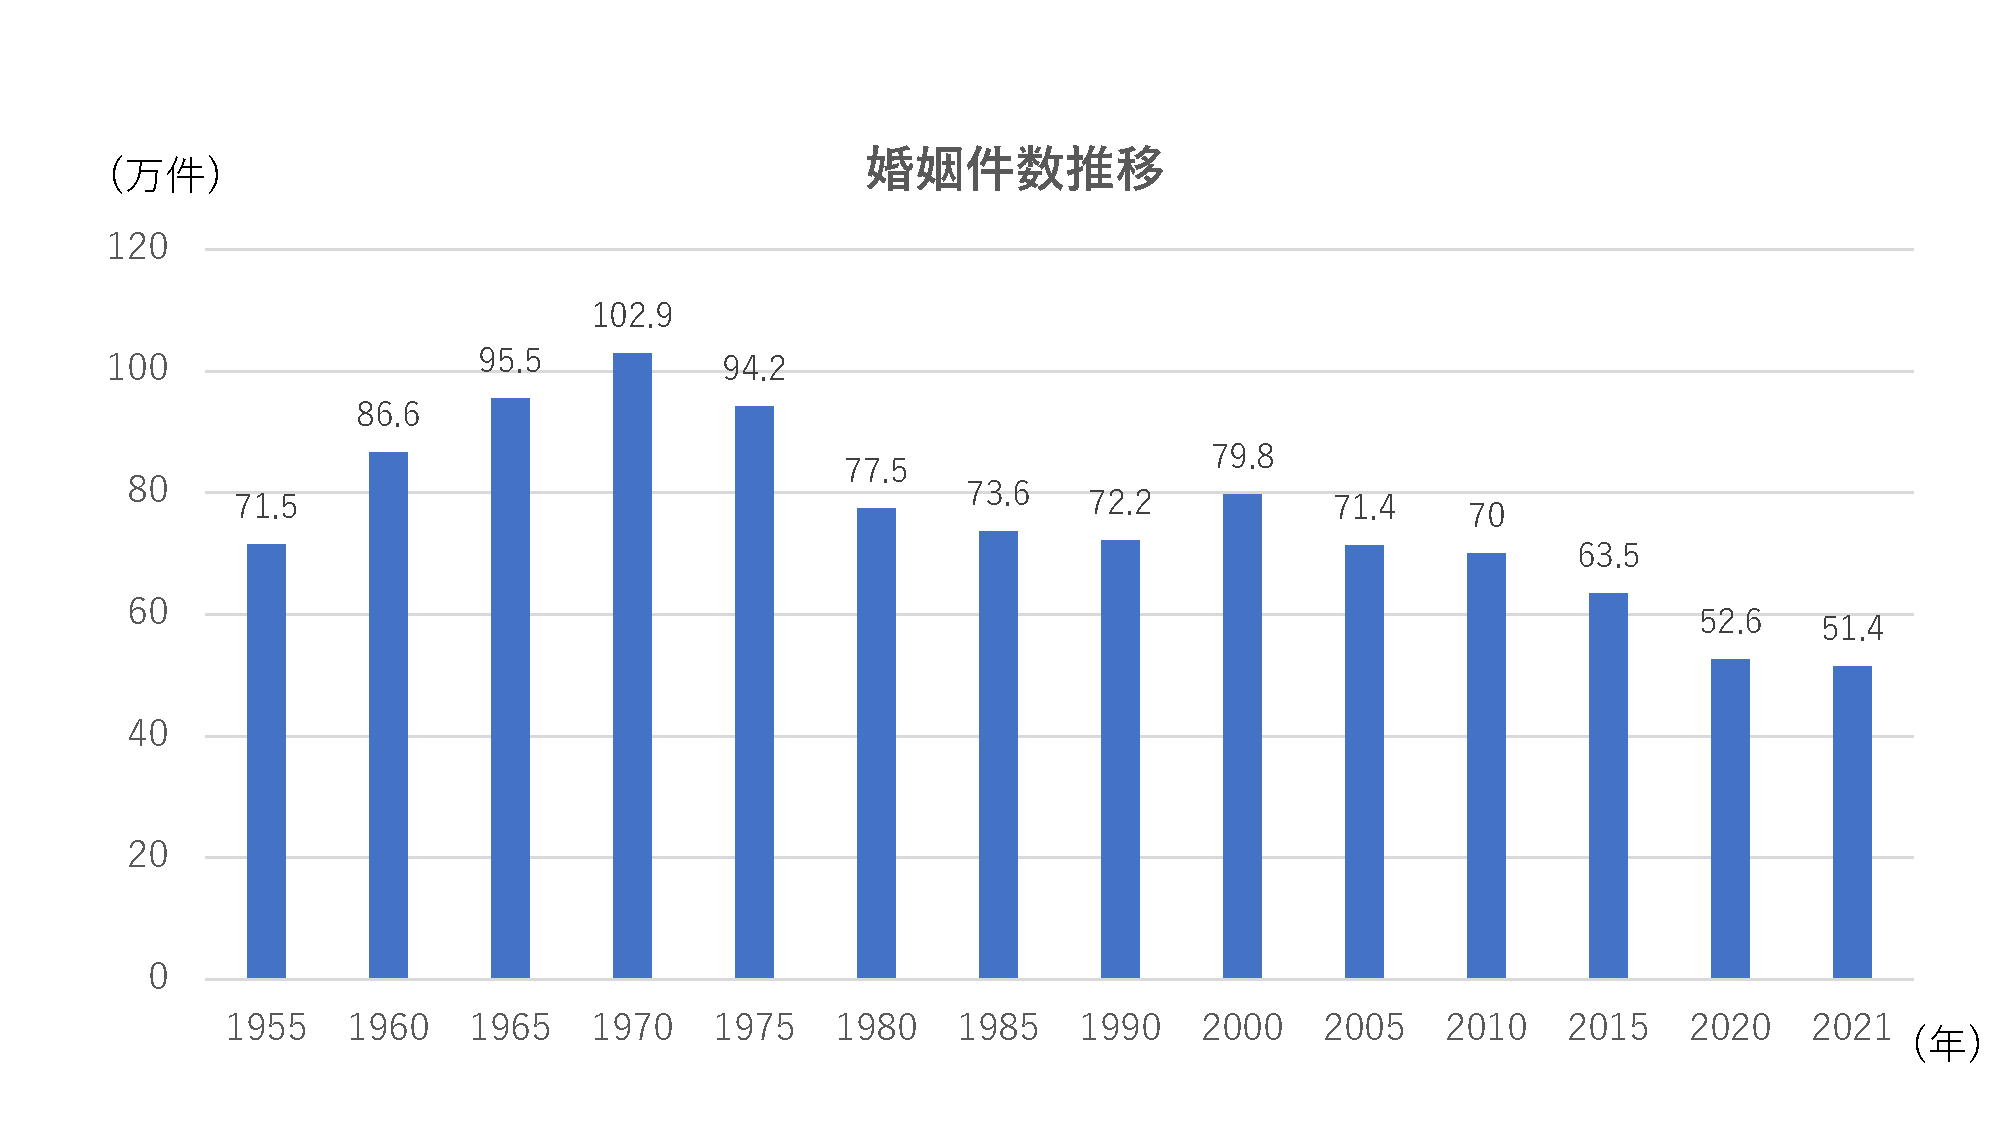
\includegraphics[keepaspectratio, scale=0.5]{koninnsuii.pdf}
\end{center}
 \caption{婚姻数の推移}
 \label{fig:konninn}
\end{figure}

\begin{figure}[h]
\begin{center}
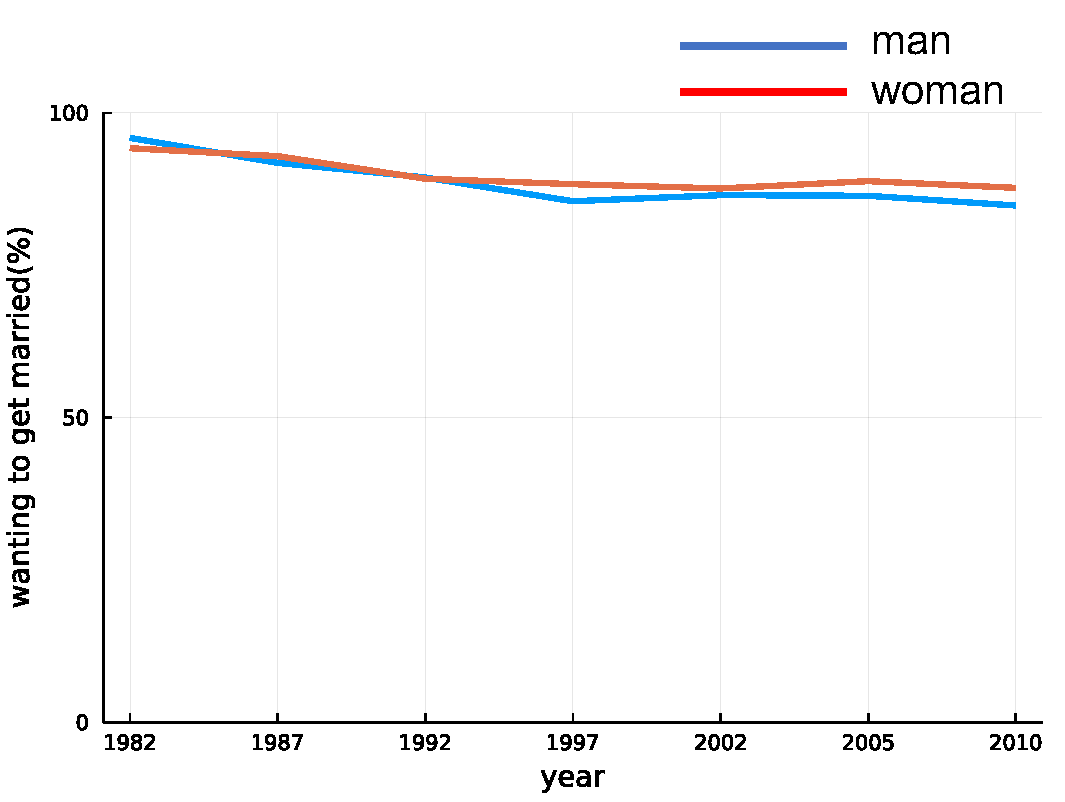
\includegraphics[keepaspectratio, scale=0.7]{preview.pdf}
\end{center}
 \caption{結婚意欲の推移}
 \label{fig:iyoku}
\end{figure}

\clearpage

\section{マッチングアプリについて}
\subsection{概要}
マッチングアプリとは異性・同性の隔てなくインターネット回線を通じてアプリに参加している不特定多数のユーザー間で出会いを作るための仕組みのことである.
\subsection{懸念点}
出会いの場の減少から,多くの社会人がマッチングアプリを利用している.
図\ref{fig:mattingu}は2022年に実施した1620人を対象とした夫婦の出会いのきっかけ調査である.約20\%がマッチングアプリで出会ったとされ,きっかけとしては最多のものとなっている\cite{huuhuutyousa}.
一方,マッチングアプリ自体に懸念を抱いている方は多く,マッチングアプリに関する印象アンケートでは「詐欺や宗教勧誘にあいそう」,「犯罪にあいそう」などの回答が多数派であった\cite{prtimes}.

\begin{figure}[h]
\begin{center}
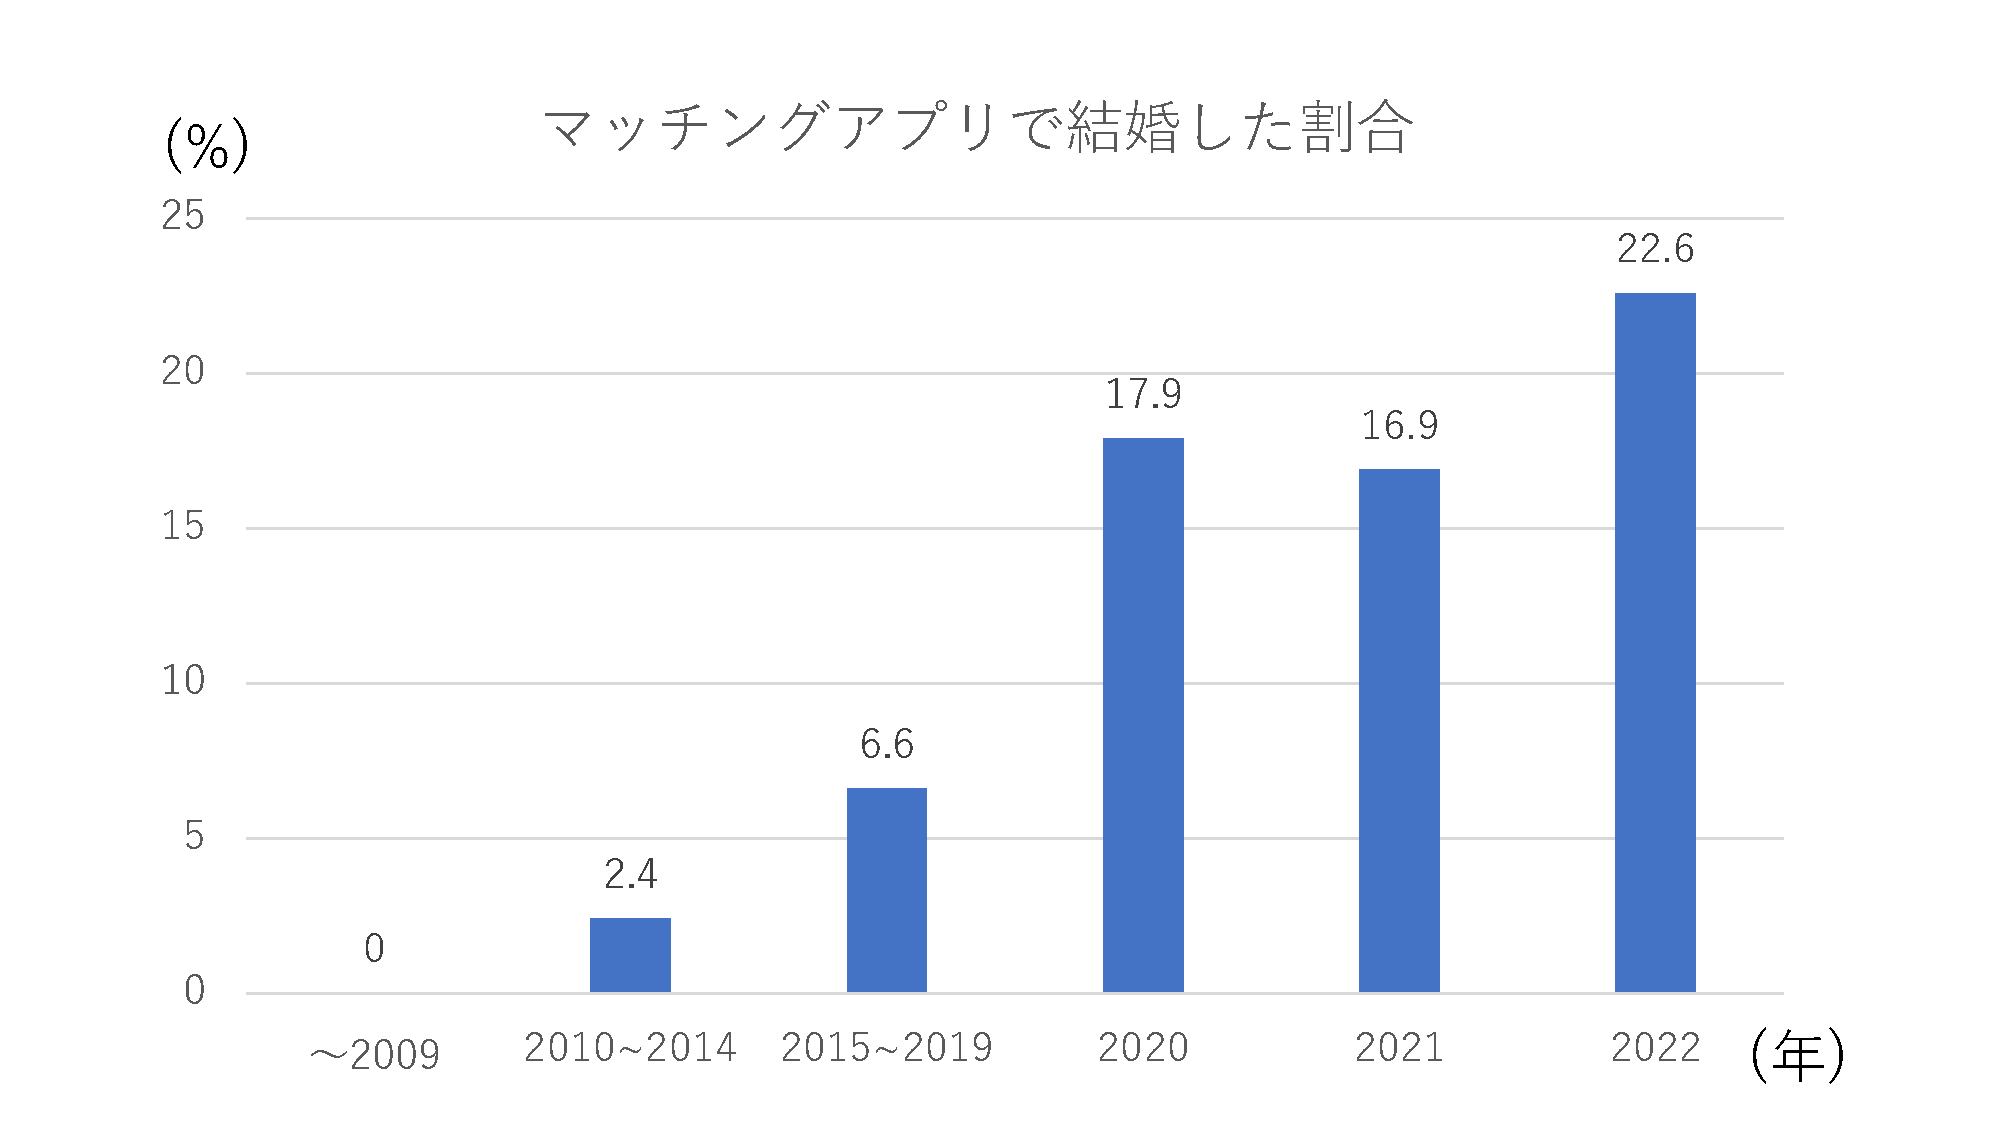
\includegraphics[keepaspectratio, scale=0.5]{mattinnguwariai.pdf}
\end{center}
 \caption{マッチングアプリで結婚した割合}
 \label{fig:mattingu}
\end{figure}
\clearpage

\section{VRデートアプリについて}
\subsection{概要}
VR間で実際のデートを模したアプリケーションである.
マッチングアプリなどで文面上のコミュニケーションは取れたが異性と直接会うことに抵抗,恐怖を持つ方,まだデート経験が少なく,エスコートに慣れていない方がデートそのものに慣れるべく開発した.

\subsection{システム概要}\label{システム概要}
VR空間内でデートするアプリでは個別の問題点を以下のように改善するコンセプトを考案する.
まず,2人きりで会うことの不安については,VR空間内で擬似的にデートを行うことで改善できる.
アプリは時間が40分〜1時間程度に設定しており,自動進行としている.
自動進行の意図としては,デートの行動の制限し筋道を建てることでデート未経験者が失敗しないように配慮をしている.
デート時間の前半に共通の体験をしてもらい,後半はその体験についておしゃべりする時間としてお互いの性格を知る機会を設けることとした.

\subsection{VR内で会話機能のある類似アプリケーションについて} 
現在VRで実装され,本アプリケーションと最も類似するアプリケーションはVRChatである.

VRChatとは,VR空間内で多人数とのコミュニケーションを交わすことができる「ソーシャルVR」と呼ばれるジャンルのアプリケーションである.
VRChat内には内にはユーザーが手がけた様々な「ワールド」と呼ばれるVR空間が用意されており、好きな場所で他のユーザーとの交流を楽しむことができる。周囲にいるプレイヤーとはボイスチャットはもちろん、自分の身体の動きをアバターに反映させ、ボディーランゲージも可能となっている.
\subsection{VRデートアプリと類似アプリケーションについて}
VRChatは,VRChatは自由度が高く出来ることが多いためデート初心者にとっては何処に行けば良いのか,何をしたら良いのかの選択肢が広く計画を立てるのが困難である.

そこで,時間に制限をつけ,デートコースを制限することで既存のアプリにはないデートをしやすい環境をつくれるのではないかと考えた.

\clearpage


\section{システム実装}
\subsection{システム設計}
この節ではどのようにアプリケーションを作成したのかについて記していく.
\subsubsection{開発手順}
本研究では,アプリケーションの作成はゲーム開発エンジンであるUnityを用いた.

\label{sec:0}
\subsubsection{VR空間の設定}
本研究の目的としてデートの不安を軽減するとある.すなわち,デート自体に慣れるということであり,実際のデートを模す必要がある.そこで,VR空間内に動きが同期している男性アバターと女性アバターを作成し,デート環境が一般的なものであるものを用意した.

図\ref{fig:screen}は作成したVR空間を示し,①,②をそれぞれ男性アバター,女性アバターとした.
また,\ref{システム概要}にあるように③の方向に自動進行していく.

\begin{figure}[h]
\begin{center}
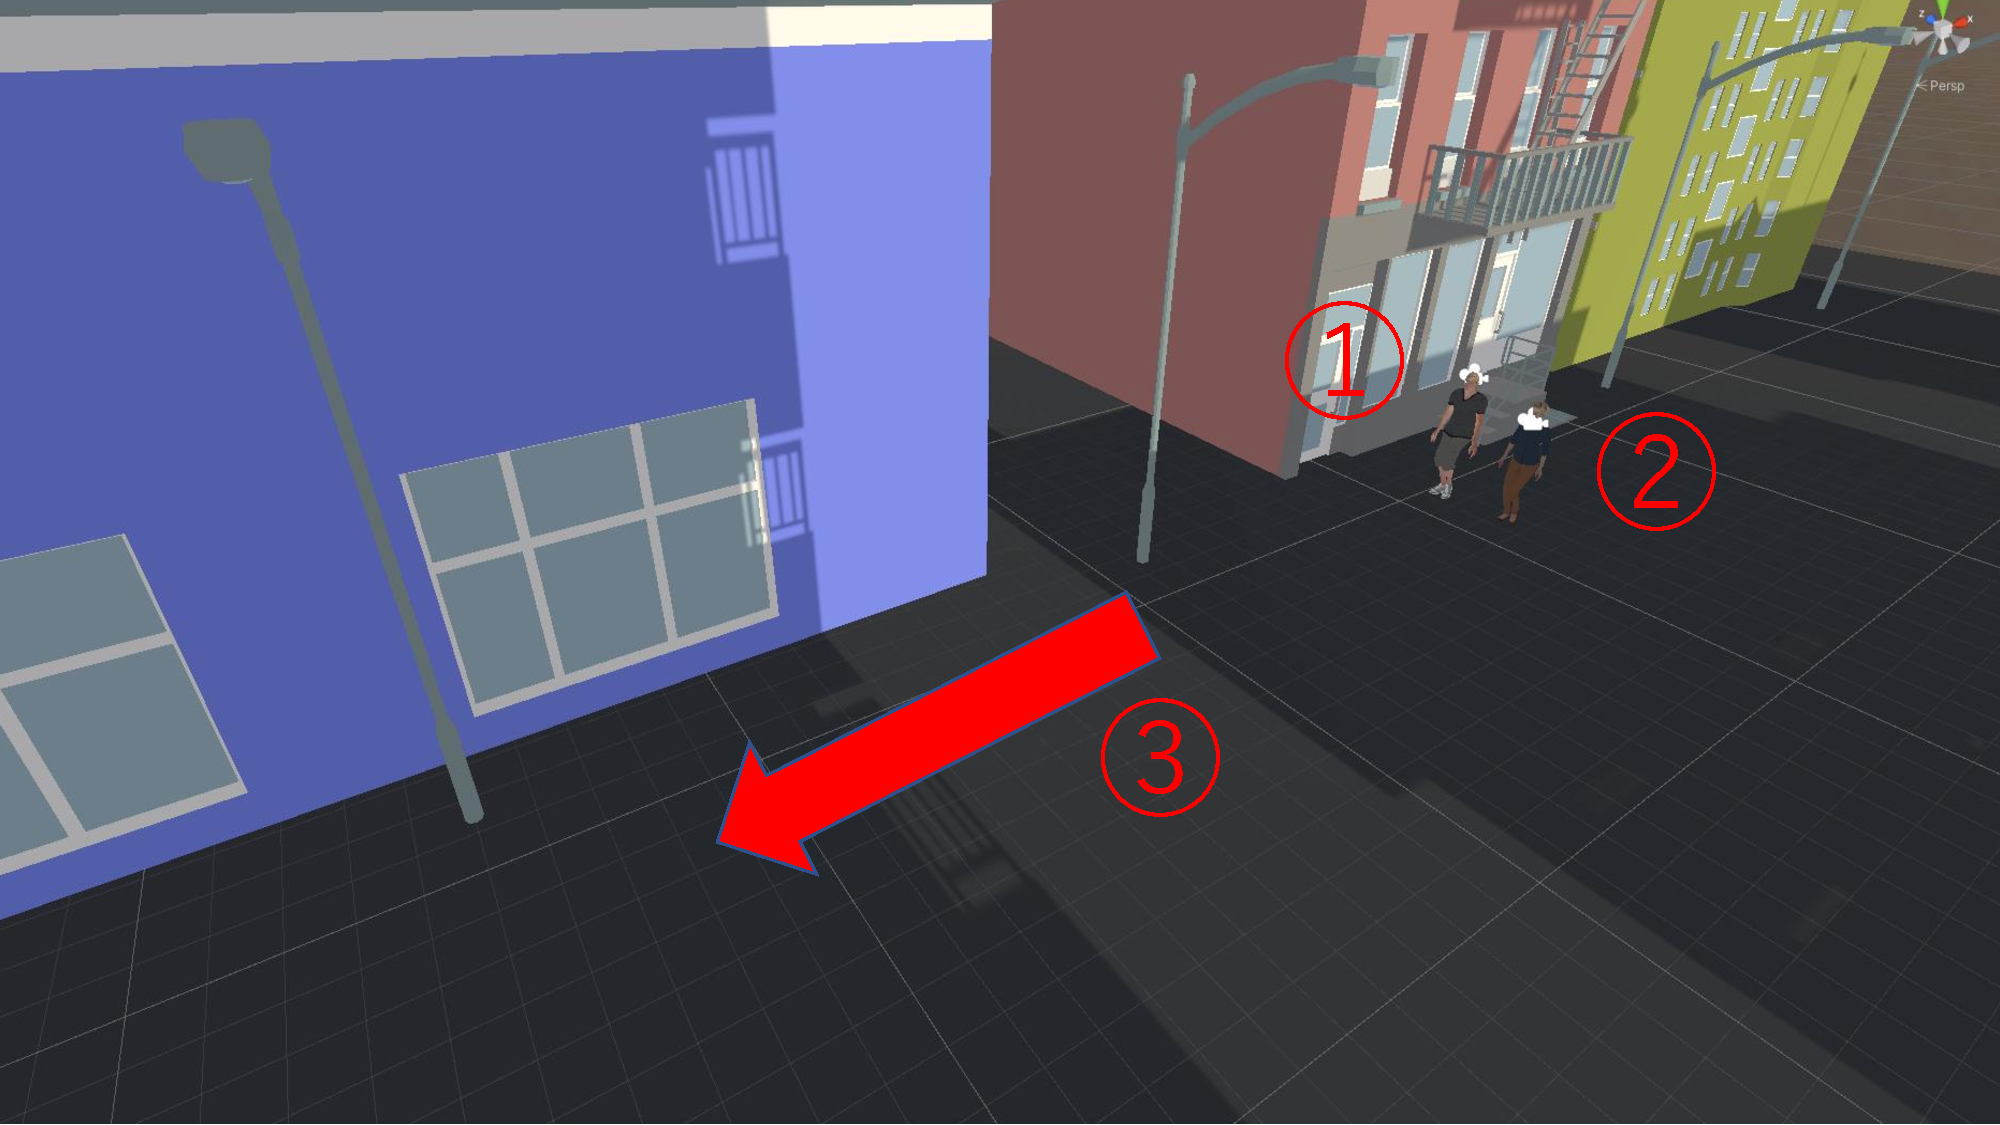
\includegraphics[keepaspectratio, scale=0.5]{screenshot.pdf}
\end{center}
 \caption{作成したVR空間}
 \label{fig:screen}
\end{figure}
\subsubsection{視点同期方法}
視点の同期はWebSocket-sharpを用いて実装した.

\clearpage

\section{VRアプリに実装した技術}
この節ではアプリに実装した技術について記している.
\subsection{SkyBox}
SkyBoxと呼ばれる空の景色を変えることができる機能を実装した.
この機能はDirectional Lightにアタッチすることで実装することができる.
また,SkyBoxのスクリプトに5種類の空の景色を入れて時間帯で入れ替わるようにすることで早朝,朝,昼,夕方,夜と現実に近い空間をつくることに成功した.

\subsection{自動進行}

\clearpage

\section{開発環境}
\subsection{使用言語}
\subsubsection{C\#}
制御構文などに高水準言語の特徴を持ちながら、ハードウェア寄りの記述も可能な低水準言語の特徴も併せ持つ。基幹系システムや、動作環境の資源制約が厳しい、あるいは実行速度性能が要求されるソフトウェアの開発に用いられることが多い。後発のC++やJava、C\#など、「C系」と呼ばれる派生言語の始祖でもある.

\subsection{使用エンジン} 
\subsubsection{Unity}
UnityとはUnity Technologiesが開発したゲーム開発プラットフォームであり,主にC\#を用いたプログラミングでコンテンツの開発が可能である。iOSやAndroid、XboxやPlayStation4などの様々なプラットフォームでの開発,VR/AR/MR機器向けのコンテンツ開発にも対応している。

\subsection{通信プロトコル}
\subsubsection{WebSocket}
WebSocketとは、ブラウザとウェブサーバーとの間で双方向通信を行うための通信プロトコルである.
サーバー側とユーザー側が常にオンライン状態を維持することによって、双方向通信を可能としている.
そのため,従来の通信プロトコルと比べ,リアルタイムに情報共有することを可能としている.
\clearpage

\section{結言}
2015年9月に開催された「国連持続可能な開発サミット」でSDGsが掲げられた.この中に少子化も含まれており,その要因は,晩婚化の進展\cite{sasaki2012},交際率・婚姻率の減少\cite{naikakufu2019}などとされている.

実際に日本では,20年間で平均初婚年齢は2.6歳(男性)/3.1歳(女性)増加している.
しかし,結婚意欲は僅かに減少している程度でほぼ変化していない.
すなわち,「結婚はしたいけれど,良い相手に恵まれない」との考えが大多数を占めている\cite{naikakufu2019}.

過去には学校や職場,友人を通じた出会いが有ったが,最近では出会いの場としてSNSを活用する者やマッチングアプリの利用者が増加している.
しかし,知らない人と2人きりで会うことに恐怖を感じたり,初デートに不安を感じるデート未経験者も少なくない\cite{prtimes,yoshimura2020}.

本研究では,異性と直接会うことに抵抗,恐怖を持つ方,まだデート経験が少なく,エスコートに慣れていない方がデートそのものに慣れるためのアプリケーションを開発した.このアプリケーションを使用することで2人きりで会う恐怖を緩和し,デートに対する不安を軽減することが期待される.また,今後このアプリケーションを使用してもらい,どの程度恐怖や不安が軽減されたのか評価してもらいたい.

\clearpage



\section{謝辞}
本研究の遂行及び本論文の作成にあたり,須田研究室の仲間に多くの手助けを頂きました,深く感謝の意を表します.そして,本論文の作成にあたり多大なる御指導及び御助言を頂きました,須田宇宙准教授に深く感謝の意を表します.

\clearpage

%参考文献
\begin{thebibliography}{99}
\bibitem{sasaki2012} 佐々木 尚之: ``不確実な時代の結婚-JGSSライフコース調査による潜在的稼得力の影響の検証'', 「家族社会学研究」,第24号,pp152-164(2012)
\bibitem{naikakufu2019} 内閣府: ``少子化対策の現状'', \url{https://www8.cao.go.jp/shoushi/shoushika/whitepaper/measures/w-2016/28webhonpen/html/b1_s1-1-3.html}, 2019/3/26参照
\bibitem{naikakufu2022} 内閣府: ``令和4年版男女共同参画白書'', \url{https://www.gender.go.jp/about_danjo/whitepaper/r04/gaiyou/pdf/r04_gaiyou.pdf}, 2022/6/14参照
\bibitem{doukou}国立社会保障・人口問題研究所:``第15回出生動向基本調査'',
\bibitem{prtimes}PRTIMES:``マッチングアプリは怖い?危ない目に合った?初めて会うまでの期間は!?徹底調査'',
\url{https://prtimes.jp/main/html/rd/p/000000016.000059676.html},2021/10/4参照
\url{https://www.ipss.go.jp/ps-doukou/j/doukou15/NFS15_report3.pdf},2022/3/14参照
\bibitem{wecsocketsetumi}WebSocketとは?WebSocketについて詳しく解説します:``Web会議の基礎知識'',
\url{https://www.freshvoice.net/knowledge/word/6323/},2022/6/10参照
\bibitem{huuhuutyousa}「いい夫婦の日」に関するアンケート調査:``明治安田生命 NEWS RELEASE'',
\url{https://www.meijiyasuda.co.jp/profile/news/release/2022/pdf/20221116_01.pdf},2023/1/16参照
\end{thebibliography}

\end{document}
